\documentclass[11pt,a4paper]{article}

\usepackage[margin=2.2cm]{geometry}
\usepackage[T1]{fontenc}
\usepackage{lmodern}
\usepackage{amssymb}
\usepackage{xcolor}
\usepackage{tikz}
\usetikzlibrary{arrows.meta,positioning,fit,shapes.geometric,backgrounds,calc}
\usepackage{booktabs}
\usepackage{tabularx}
\usepackage{enumitem}
\usepackage{listings}
\usepackage[most]{tcolorbox}
\usepackage{titlesec}
\usepackage{fancyhdr}
\usepackage[colorlinks=true,linkcolor=blue!50!black,urlcolor=blue!50!black]{hyperref}

% ---------- colours ----------
\definecolor{local}{HTML}{2E7D32}
\definecolor{cloud}{HTML}{1565C0}
\definecolor{warn}{HTML}{C62828}
\definecolor{idea}{HTML}{6A1B9A}
\definecolor{soft}{HTML}{F5F5F5}

% ---------- boxes ----------
\newtcolorbox{concept}[1]{colback=idea!4,colframe=idea!70,fonttitle=\bfseries,title={Concept: #1},breakable}
\newtcolorbox{analogy}{colback=local!5,colframe=local!70,fonttitle=\bfseries,title={Analogy},breakable}
\newtcolorbox{why}{colback=cloud!4,colframe=cloud!70,fonttitle=\bfseries,title={Why we chose this},breakable}
\newtcolorbox{caution}{colback=warn!4,colframe=warn!70,fonttitle=\bfseries,title={Watch out},breakable}
\newtcolorbox{exercise}{colback=soft,colframe=black!50,fonttitle=\bfseries,title={Check yourself},breakable}

\lstset{basicstyle=\ttfamily\small,backgroundcolor=\color{soft},frame=single,
        rulecolor=\color{black!25},columns=fullflexible,keepspaces=true,
        showstringspaces=false,breaklines=true}

\pagestyle{fancy}
\fancyhf{}
\lhead{\small Listen -- Learning Doc 01}
\rhead{\small System Architecture Intuition}
\cfoot{\thepage}

\title{\textbf{Listen}\\[4pt]\large Learning Doc 01: System Architecture Intuition}
\author{Written while designing the project, before any code exists}
\date{4 October 2026}

\begin{document}
\maketitle

\begin{abstract}
\noindent This document explains \emph{how} and \emph{why} the Listen system is shaped the
way it is. Listen is a lightweight Windows voice assistant: it listens for commands, tracks
which apps you use, carries out actions like ``search what is an atom'', and shows your
analytics in a web app. You will not find code here. You will find the reasoning that comes
\emph{before} code, which is the part most tutorials skip and the part that matters most when
a project grows.
\end{abstract}

\tableofcontents
\newpage

% =====================================================================
\section{What is ``system architecture''?}

\begin{concept}{System architecture}
The \textbf{architecture} of a software system is the set of decisions about
\begin{enumerate}[nosep]
  \item \textbf{what the big pieces are} (components),
  \item \textbf{where each piece runs} (your laptop? a server?),
  \item \textbf{how the pieces talk to each other} (function calls? the internet?), and
  \item \textbf{where data lives} and who is allowed to see it.
\end{enumerate}
Architecture is about the decisions that are \emph{expensive to change later}. The colour
of a button is not architecture. Whether your audio is processed on your laptop or in the
cloud \emph{is}.
\end{concept}

\begin{analogy}
Think of building a house. Before laying a single brick, an architect decides: how many
floors, where the kitchen goes, where the plumbing runs. You can repaint a wall any time.
Moving the plumbing after the house is built means tearing up floors. Software is the same:
architecture is the plumbing.
\end{analogy}

\subsection{Why decide before coding?}
Beginners often start by writing code and ``figuring it out as they go''. That works for a
100-line script. For a project with several parts (a voice agent, a usage tracker, an API,
a web app) it usually ends with a rewrite, because two parts were built on incompatible
assumptions. Ten minutes of thinking on paper saves days of untangling code.

% =====================================================================
\section{Architecture starts from requirements}

You cannot judge an architecture as ``good'' in the abstract. It is only good \emph{for a
particular set of requirements}. Engineers split requirements into two kinds:

\begin{concept}{Functional vs.\ non-functional requirements}
\textbf{Functional} requirements say \emph{what the system does}: ``when I say
\emph{search X}, open Google and search X''.

\textbf{Non-functional} requirements say \emph{how well / under what limits} it does it:
``it must be lightweight'', ``my private conversations must not leave my laptop'', ``it
must work offline''.

Non-functional requirements shape the architecture the most. Almost any design can
\emph{eventually} open Google; far fewer can do it in 200\,MB of RAM, offline, privately.
\end{concept}

\subsection{Listen's requirements}

\noindent\textbf{Functional:}
\begin{itemize}[nosep]
  \item Listen through the microphone in three modes: wake word (default), continuous
        transcription (toggle), push-to-talk hotkey (fallback).
  \item Understand commands: \texttt{open}, \texttt{search}, \texttt{close}, \texttt{volume},
        \texttt{play \{query\} on youtube}, with \emph{default apps} when none is named.
  \item Let you add and edit commands \emph{without touching code}, helped by an AI
        ``command builder''.
  \item Track which apps (and, from window titles, which websites) you use.
  \item Show analytics in a full web app; expose a documented API.
\end{itemize}

\noindent\textbf{Non-functional (the ones that drive the design):}
\begin{itemize}[nosep]
  \item \textbf{Lightweight}: runs all day on a 16\,GB laptop with integrated graphics.
  \item \textbf{Private}: raw transcripts and raw window titles never leave the laptop.
  \item \textbf{Works offline}: commands still work and nothing is lost without internet.
  \item \textbf{Extensible}: new commands, speech engines and listening modes plug in.
  \item \textbf{Learnable}: this is a first project, so debuggability beats cleverness.
\end{itemize}

Keep this list in mind. Every decision below points back to one of these lines.

% =====================================================================
\section{The first big split: what \emph{must} run where}

Some decisions are made for you by physics. A server in a data centre cannot hear your
microphone, and it cannot see which window is open on your screen. So:

\begin{itemize}
  \item The \textcolor{local}{\textbf{voice agent}} and \textcolor{local}{\textbf{usage agent}}
        \emph{must} run on your laptop.
  \item The \textcolor{cloud}{\textbf{web app}} and \textcolor{cloud}{\textbf{API}} should run
        on a server, so you can open your dashboard from any device, and so they can be
        \emph{deployed}.
\end{itemize}

\begin{concept}{Client and server}
A \textbf{server} is a program that waits for requests and answers them (e.g.\ ``give me my
app-usage stats for this week''). A \textbf{client} is a program that sends those requests.
The same machine can be both. In Listen, the laptop agent and the React web app are both
\emph{clients} of the cloud API.
\end{concept}

This one observation already gives us the outline of the whole system: a \textbf{local
side} and a \textbf{cloud side}, connected over the internet.

% =====================================================================
\section{The three candidate architectures}

Given ``local side + cloud side'', the open question was \emph{how to organise the local
side}. We compared three options.

\subsection{Option 1: Modular monolith + cloud hub \quad(\textcolor{local}{chosen})}

\begin{concept}{Monolith}
A \textbf{monolith} is a single program (one process) that contains all the features.
A \textbf{modular} monolith is still one program, but its inside is split into clearly
separated modules that only talk through well-defined interfaces. You get the simplicity of
one program with most of the organisation of separate services.
\end{concept}

On the laptop, one Python process contains a voice module, a usage module, an action
executor, a local database and a sync client. The modules run on separate \emph{threads} and
communicate through an in-memory \emph{event bus} (Section~\ref{sec:inside}).

\subsection{Option 2: Microservices with a message broker}

\begin{concept}{Microservices}
\textbf{Microservices} split a system into many small, \emph{separate programs}, each doing
one job, talking over a network or a \textbf{message broker} (a program whose only job is
passing messages between other programs, e.g.\ Redis, RabbitMQ).
\end{concept}

The voice agent, usage agent and executor would each be their own Python program. If one
crashes, the others keep running. But every Python program carries its own interpreter and
libraries in memory (tens of MB each), plus the broker itself. That directly contradicts
the \emph{lightweight} requirement. It is also much harder to debug: one bug might involve
three programs and their message traffic. Microservices mostly solve an \emph{organisational}
problem: many teams working on one product without stepping on each other. We are one
person.

\subsection{Option 3: Thin local agent, everything in the cloud}

The laptop would keep no data of its own and send every event straight to the cloud API.
That is the simplest code, but it breaks \emph{offline} (no internet means lost events and
no command list) and \emph{privacy} (everything leaves the laptop by default).

\subsection{Side-by-side}

\begin{center}
\renewcommand{\arraystretch}{1.25}
\begin{tabularx}{\textwidth}{l X X X}
\toprule
 & \textbf{1. Modular monolith} & \textbf{2. Microservices} & \textbf{3. Thin agent} \\
\midrule
Lightweight      & \textcolor{local}{Best: one process}  & \textcolor{warn}{Worst: many processes + broker} & \textcolor{local}{Good} \\
Works offline    & \textcolor{local}{Yes (local DB)}     & \textcolor{local}{Yes}           & \textcolor{warn}{No} \\
Privacy          & \textcolor{local}{Selective sync}     & \textcolor{local}{Possible}      & \textcolor{warn}{Everything uploads} \\
Debuggability    & \textcolor{local}{One terminal}       & \textcolor{warn}{Hard}           & \textcolor{local}{Easy} \\
Crash isolation  & Medium (guarded modules) & \textcolor{local}{Best}  & Medium \\
Can evolve later & \textcolor{local}{Yes: modules can be split out} & n/a & \textcolor{warn}{Needs redesign} \\
\bottomrule
\end{tabularx}
\end{center}

\begin{why}
Option 1 is the only one that satisfies \emph{all three} hard requirements at once:
lightweight, offline-capable and private. Its main weakness (one bad crash takes the
whole agent down) is handled by wrapping each module in error handling, which is far
cheaper than running a microservice fleet. And because the modules have clean boundaries,
if one ever needs to become its own process, that is a small change instead of a rewrite.
\end{why}

\begin{caution}
``Microservices'' sounds more impressive, and many tutorials push it. Picking an
architecture for how it sounds, instead of for your requirements, is one of the most common
mistakes in software. Start with the simplest design that meets the requirements;
split things later \emph{only} when a real problem appears.
\end{caution}

% =====================================================================
\section{The full picture}

\begin{center}
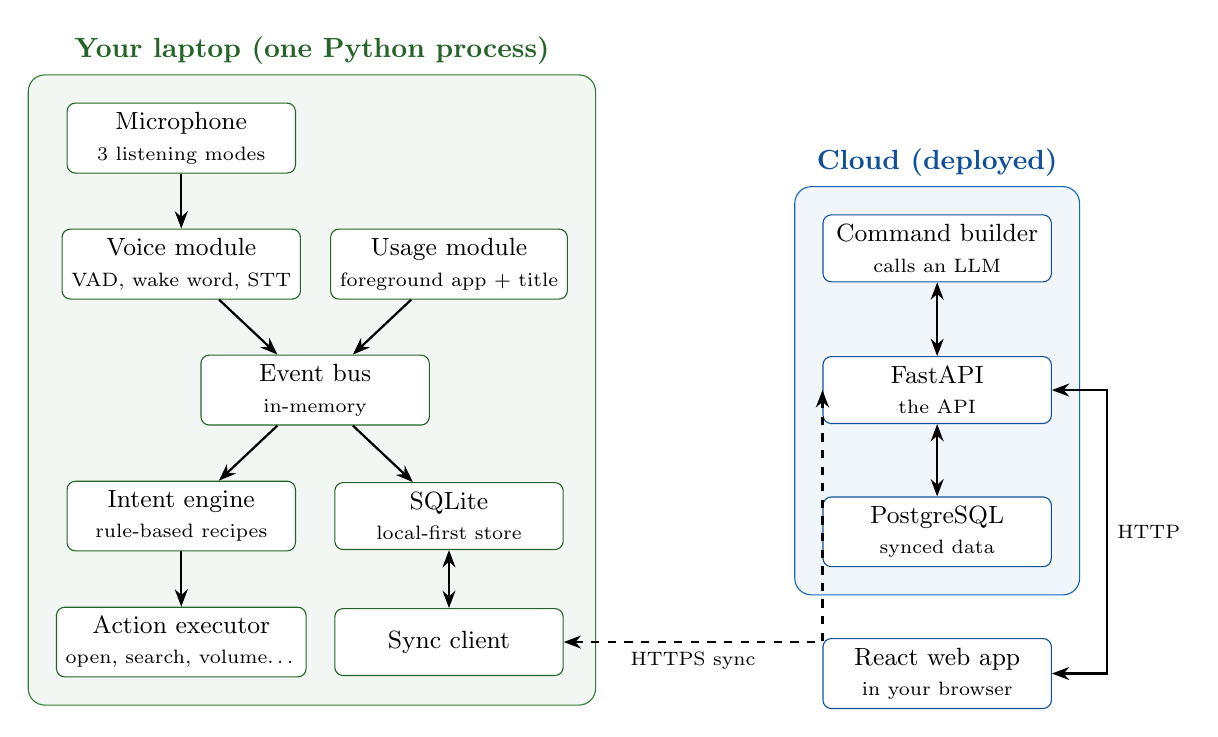
\begin{tikzpicture}[
  font=\small,
  box/.style={draw,rounded corners=3pt,minimum width=2.9cm,minimum height=0.85cm,align=center,fill=white},
  lbox/.style={box,draw=local!80!black},
  cbox/.style={box,draw=cloud!80!black},
  arr/.style={-{Stealth[length=2.2mm]},thick},
  darr/.style={{Stealth[length=2.2mm]}-{Stealth[length=2.2mm]},thick}
]
% local side
\node[lbox] (mic)   at (0,0)      {Microphone\\\scriptsize 3 listening modes};
\node[lbox] (voice) at (0,-1.6)   {Voice module\\\scriptsize VAD, wake word, STT};
\node[lbox] (usage) at (3.4,-1.6) {Usage module\\\scriptsize foreground app + title};
\node[lbox] (bus)   at (1.7,-3.2) {Event bus\\\scriptsize in-memory};
\node[lbox] (intent)at (0,-4.8)   {Intent engine\\\scriptsize rule-based recipes};
\node[lbox] (exec)  at (0,-6.4)   {Action executor\\\scriptsize open, search, volume\ldots};
\node[lbox] (db)    at (3.4,-4.8) {SQLite\\\scriptsize local-first store};
\node[lbox] (sync)  at (3.4,-6.4) {Sync client};

\draw[arr] (mic) -- (voice);
\draw[arr] (voice) -- (bus);
\draw[arr] (usage) -- (bus);
\draw[arr] (bus) -- (intent);
\draw[arr] (intent) -- (exec);
\draw[arr] (bus) -- (db);
\draw[darr] (db) -- (sync);

\begin{scope}[on background layer]
\node[draw=local,fill=local!6,rounded corners=6pt,inner sep=10pt,
      fit=(mic)(voice)(usage)(bus)(intent)(exec)(db)(sync),
      label={[text=local!80!black,font=\bfseries]above:Your laptop (one Python process)}] (L) {};
\end{scope}

% cloud side
\node[cbox] (api)   at (9.6,-3.2) {FastAPI\\\scriptsize the API};
\node[cbox] (pg)    at (9.6,-5.0) {PostgreSQL\\\scriptsize synced data};
\node[cbox] (llm)   at (9.6,-1.4) {Command builder\\\scriptsize calls an LLM};
\node[cbox] (react) at (9.6,-6.8) {React web app\\\scriptsize in your browser};

\draw[darr] (api) -- (pg);
\draw[darr] (api) -- (llm);
\draw[darr] (react.east) -- ++(0.7,0) |- node[pos=0.25,right,font=\scriptsize]{HTTP} (api.east);
\begin{scope}[on background layer]
\node[draw=cloud,fill=cloud!6,rounded corners=6pt,inner sep=10pt,
      fit=(api)(pg)(llm),
      label={[text=cloud!80!black,font=\bfseries]above:Cloud (deployed)}] (C) {};
\end{scope}

\draw[darr,dashed] (sync.east) -- node[below,sloped,font=\scriptsize]{HTTPS sync} (api.west |- sync.east) -- (api.west);
\end{tikzpicture}
\end{center}

\noindent\textbf{How to read this diagram.} Green is your laptop, blue is the cloud. Solid
arrows are function calls inside one program; the dashed arrow is network traffic over the
internet. The React app runs in your browser and talks \emph{only} to the API over HTTP;
it never touches the database directly.

% =====================================================================
\section{Inside the local agent}\label{sec:inside}

\subsection{Modules and threads}
\begin{concept}{Thread}
A \textbf{thread} is a sequence of instructions running inside a program. One program can
have several threads, so the voice module can wait for audio \emph{while} the usage module
checks the foreground window every few seconds. Threads share the program's memory, so
they are much lighter than separate programs.
\end{concept}

\subsection{The event bus}
\begin{concept}{Event bus (publish / subscribe)}
Instead of modules calling each other directly, a module \textbf{publishes} an
\emph{event} (``command heard: \texttt{search what is an atom}''), and any module that
\textbf{subscribed} to that kind of event gets it. The publisher does not know or care who
is listening.
\end{concept}

\begin{analogy}
A radio station broadcasts; anyone with a radio tuned in hears it. The station does not
keep a list of listeners. If you add a new listener (say, an ``analytics logger''), the
station does not change at all.
\end{analogy}

\begin{why}
Without a bus, the voice module would need to know about the intent engine, the database
and the logger, and every new feature would mean editing the voice module. With a bus, new
features just subscribe. This is called \textbf{loose coupling}: parts depend on a shared
message format instead of on each other.
\end{why}

\subsection{Pluggable pieces (one interface, many implementations)}

You asked for three listening modes, two kinds of speech engine, and two ways to build
commands. All of these follow one pattern:

\begin{concept}{Interface + interchangeable implementations}
Define \emph{what} a piece must do (its \textbf{interface}), for example ``a
\texttt{SpeechEngine} takes audio and returns text''. Then write several pieces that all
honour it: \texttt{FasterWhisperEngine}, \texttt{CloudEngine}. The rest of the program only
talks to the interface, so swapping one engine for another is a setting, not a rewrite.
(Textbooks call this the \emph{strategy pattern}.)
\end{concept}

\begin{center}
\renewcommand{\arraystretch}{1.2}
\begin{tabularx}{\textwidth}{l X}
\toprule
\textbf{Interface} & \textbf{Implementations in Listen} \\
\midrule
\texttt{AudioTrigger}   & Wake word (default) \quad$\cdot$\quad Continuous \quad$\cdot$\quad Push-to-talk hotkey \\
\texttt{SpeechEngine}   & faster-whisper (offline, default) \quad$\cdot$\quad Cloud STT (optional) \\
\texttt{CommandBuilder} & LLM builder (online) \quad$\cdot$\quad Guided form (offline fallback) \\
\texttt{Shell}          & Terminal (v1) \quad$\cdot$\quad System tray app (later) \\
\bottomrule
\end{tabularx}
\end{center}

Notice the last row: ``terminal first, tray later'' is not a rewrite. The tray is just a
different \emph{shell} around the same core.

\subsection{Keeping it lightweight}
The single most important trick is a \textbf{gate}: cheap work runs all the time,
expensive work runs only when the cheap work says it is needed.

\begin{center}
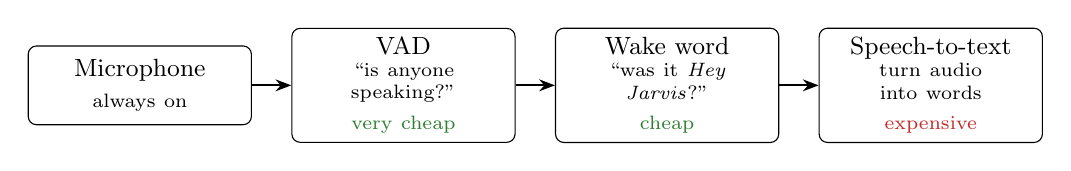
\begin{tikzpicture}[font=\small,
  st/.style={draw,rounded corners=3pt,align=center,minimum height=1cm,text width=2.6cm,fill=white},
  arr/.style={-{Stealth[length=2mm]},thick}]
\node[st] (a) {Microphone\\\scriptsize always on};
\node[st,right=0.5cm of a] (b) {VAD\\\scriptsize ``is anyone speaking?''\\\scriptsize\textcolor{local}{very cheap}};
\node[st,right=0.5cm of b] (c) {Wake word\\\scriptsize ``was it \emph{Hey Jarvis}?''\\\scriptsize\textcolor{local}{cheap}};
\node[st,right=0.5cm of c] (d) {Speech-to-text\\\scriptsize turn audio into words\\\scriptsize\textcolor{warn}{expensive}};
\draw[arr] (a)--(b); \draw[arr] (b)--(c); \draw[arr] (c)--(d);
\end{tikzpicture}
\end{center}

\begin{concept}{VAD (voice activity detection)}
A tiny model that answers only one question: ``is this sound a human voice?''. Silence,
fans and keyboard clicks are thrown away before anything expensive runs. In continuous
mode the wake-word step is skipped, so VAD is what keeps continuous mode affordable.
\end{concept}

\noindent The exact memory and CPU numbers depend on the models we pick, so we will
\emph{measure} them on your laptop during the build instead of trusting estimates.

% =====================================================================
\section{Commands are data, not code}

This is the idea that makes ``add a command without touching code'' possible.

The Python code knows only a small, fixed set of \textbf{action primitives}:
\texttt{open\_url}, \texttt{launch\_app}, \texttt{close\_app}, \texttt{set\_volume},
\texttt{press\_keys}. Every command is a \emph{recipe} that combines a pattern with one of
these primitives, stored in a data file:

\begin{lstlisting}
- pattern: "search {query}"
  action: open_url
  target: "{default:search}"          # filled from your defaults

- pattern: "play {query} on spotify"
  action: open_url
  target: "https://open.spotify.com/search/{query}"
\end{lstlisting}

\begin{analogy}
A kitchen has a fixed set of appliances (oven, blender, stove): those are the primitives.
Recipes are written on cards: those are the commands. Adding a new dish means writing a new
card, not buying a new oven. The AI command builder is a helper who writes the card for you;
you read it and approve it before it goes in the box.
\end{analogy}

\begin{caution}
The limit: a command that needs a \emph{new kind of action} (for example, controlling smart
lights) needs a new primitive, and that is code. Anything built from existing primitives
needs none.
\end{caution}

\paragraph{Defaults.} Each verb (\texttt{search}, \texttt{play}) has a default target. The
usage module \emph{suggests} defaults from your history (``you search on Google most''),
and you can override them in settings. ``\texttt{play lofi}'' with no app named goes to
YouTube because YouTube is the default for \texttt{play}.

% =====================================================================
\section{Data: local-first with selective sync}

\begin{concept}{Local-first}
Every piece of data is written to a database \emph{on your laptop} first. The internet is
treated as optional: when it is available, data is synchronised; when it is not, nothing
breaks and nothing is lost.
\end{concept}

\subsection{Two databases, two jobs}
\begin{center}
\renewcommand{\arraystretch}{1.2}
\begin{tabularx}{\textwidth}{l X X}
\toprule
 & \textbf{SQLite (laptop)} & \textbf{PostgreSQL (cloud)} \\
\midrule
What it is & A database that is just one file; no server process & A full database server \\
Why here   & Zero setup, almost zero memory: ideal for a lightweight agent & Handles many connections; standard for deployed APIs \\
Holds      & Everything, including private data & Only what you chose to sync \\
\bottomrule
\end{tabularx}
\end{center}

\subsection{What syncs and what stays}
\begin{center}
\renewcommand{\arraystretch}{1.2}
\begin{tabularx}{\textwidth}{X c c}
\toprule
\textbf{Data} & \textbf{Stays on laptop} & \textbf{Synced to cloud} \\
\midrule
Commands you gave and their results     &  & \checkmark \\
App-usage totals (``Chrome: 3h 12m'')   &  & \checkmark \\
Cleaned site names (``Google Search'')  &  & \checkmark \\
Raw continuous-mode transcripts         & \checkmark (auto-purged after $N$ days) & \\
Raw window titles                       & \checkmark (auto-purged after $N$ days) & \\
\bottomrule
\end{tabularx}
\end{center}

\subsection{Sync goes both ways}
\begin{itemize}[nosep]
  \item \textbf{Up} (laptop $\to$ cloud): command log and usage summaries, every few minutes.
  \item \textbf{Down} (cloud $\to$ laptop): commands and settings you edited in the web app.
\end{itemize}

\begin{concept}{Source of truth}
When the same data exists in two places, you must decide which copy wins if they disagree.
For Listen: the \textbf{laptop} is the source of truth for \emph{events} (what you said,
what you used); the \textbf{cloud} is the source of truth for the \emph{command library and
settings}. Offline edits are queued and sent when the connection returns. The detailed
conflict rules come in the data design step.
\end{concept}

\begin{why}
This gives you a deployed dashboard with all the interesting analytics, while the most
sensitive data (other people's conversations, your email subjects in window titles) never
leaves your machine. If the server were ever breached, the damage is limited by design.
\end{why}

% =====================================================================
\section{The cloud side}

\begin{itemize}
  \item \textbf{FastAPI} (Python): the API. It receives sync data, serves analytics,
        stores the command library, and runs the AI command builder. It generates its own
        interactive documentation, so the API is usable by others with no extra work.
  \item \textbf{PostgreSQL}: the cloud database.
  \item \textbf{React}: the web app (dashboard, command manager, settings). It is a separate
        program that only talks to the API over HTTP, exactly like any third-party client.
\end{itemize}

\begin{concept}{API-first}
Build the API as if strangers will use it, then make your own web app its first customer.
If your own app can do everything through the API, the API is genuinely complete, and
multi-user support later (each person with their own laptop agent) becomes an extension,
not a redesign.
\end{concept}

\paragraph{Why the command builder lives in the cloud.} The web app's command manager needs
it, and the LLM's secret API key is safer on one server than copied around. When you are
offline, the laptop falls back to the guided form, so you are never blocked.

\paragraph{Future-proofing, cheaply.} Every stored record carries a \texttt{user\_id} from
day one, even though you are the only user. Adding that column now costs one line; adding it
later means migrating every table. Rule of thumb: \emph{pay small costs early only when they
prevent a painful rewrite later.} Do not build the multi-user features themselves until you
need them; that principle is called \textbf{YAGNI} (``You Aren't Gonna Need It'').

% =====================================================================
\section{Walkthrough: the life of one command}

You say: \emph{``Hey Jarvis \ldots search what is an atom''}.

\begin{enumerate}
  \item \textbf{Microphone} streams audio into the voice module.
  \item \textbf{VAD} notices human speech and passes those chunks on.
  \item \textbf{Wake-word model} recognises ``Hey Jarvis'' and opens a recording window of a
        few seconds.
  \item \textbf{Speech engine} (faster-whisper) turns that audio into the text
        \texttt{"search what is an atom"}.
  \item The voice module \textbf{publishes} a \texttt{CommandHeard} event on the bus.
  \item The \textbf{intent engine} matches it to the recipe \texttt{search \{query\}} with
        \texttt{query = "what is an atom"}. The target is the default for \texttt{search}:
        Google.
  \item The \textbf{action executor} runs the primitive \texttt{open\_url} with\\
        \url{https://www.google.com/search?q=what+is+an+atom}.
  \item A \texttt{CommandExecuted} event is published; the \textbf{database} subscriber
        writes it to SQLite.
  \item A few minutes later the \textbf{sync client} uploads it to the API, and it appears
        in your \textbf{dashboard}.
\end{enumerate}

\noindent Every step is a separate, testable piece. When something goes wrong, the terminal
shows exactly which step failed. That is the payoff of the architecture.

% =====================================================================
\section{How projects are built (and where we are)}

\begin{center}
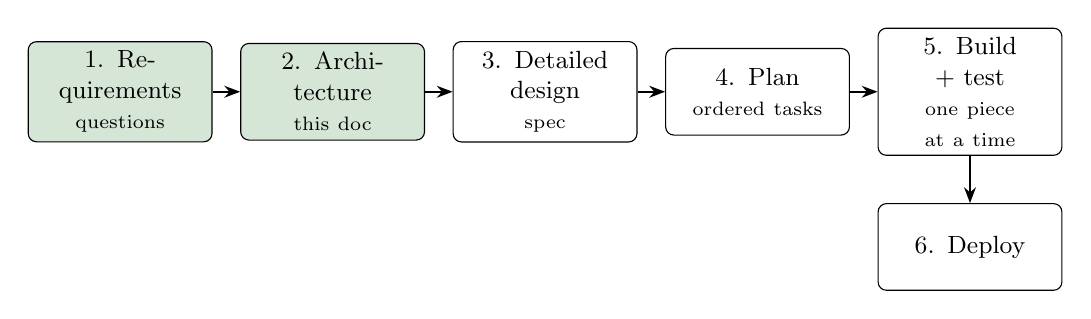
\begin{tikzpicture}[font=\small,
  ph/.style={draw,rounded corners=3pt,align=center,minimum height=1.1cm,text width=2.1cm},
  arr/.style={-{Stealth[length=2mm]},thick}]
\node[ph,fill=local!20] (p1) {1. Requirements\\\scriptsize questions};
\node[ph,fill=local!20,right=0.35cm of p1] (p2) {2. Architecture\\\scriptsize this doc};
\node[ph,right=0.35cm of p2] (p3) {3. Detailed design\\\scriptsize spec};
\node[ph,right=0.35cm of p3] (p4) {4. Plan\\\scriptsize ordered tasks};
\node[ph,right=0.35cm of p4] (p5) {5. Build + test\\\scriptsize one piece at a time};
\node[ph,below=0.6cm of p5] (p6) {6. Deploy};
\draw[arr] (p1)--(p2); \draw[arr] (p2)--(p3); \draw[arr] (p3)--(p4); \draw[arr] (p4)--(p5); \draw[arr] (p5)--(p6);
\end{tikzpicture}
\end{center}

\noindent Green phases are done. Real teams loop back: building often reveals something the
design missed, and that is normal. The goal of design is not to predict everything; it is to
make the \emph{expensive} decisions deliberately, so that the surprises are cheap ones.

\paragraph{Planned build order.} Each stage produces something you can run and see:
\begin{enumerate}[nosep]
  \item Voice agent in the terminal (wake word $\to$ text $\to$ command $\to$ action).
  \item Usage agent + local SQLite.
  \item FastAPI + PostgreSQL, sync client.
  \item React web app (dashboard, command manager, settings), AI command builder.
  \item Tray app, then deployment.
\end{enumerate}

% =====================================================================
\section{Glossary}
\begin{description}[style=nextline,leftmargin=1.2cm,itemsep=2pt]
  \item[API] A defined set of requests a program accepts, so other programs can use it.
  \item[Client / server] The program that asks / the program that answers.
  \item[Event bus] A shared channel where modules publish events and others subscribe.
  \item[Interface] A promise about what a component does, without saying how.
  \item[Local-first] Data lives on your device first; the network is optional.
  \item[Loose coupling] Parts depend on shared message formats, not on each other.
  \item[Microservices] A system made of many separate small programs.
  \item[Modular monolith] One program, internally split into well-separated modules.
  \item[Non-functional requirement] A quality limit: speed, memory, privacy, offline.
  \item[Primitive] One of the few basic actions the code knows how to perform.
  \item[Source of truth] The copy of the data that wins when copies disagree.
  \item[STT] Speech-to-text.
  \item[Thread] A line of execution inside a program; several can run at once.
  \item[VAD] Voice activity detection: ``is this sound a human voice?''.
  \item[YAGNI] ``You Aren't Gonna Need It'': do not build features before you need them.
\end{description}

% =====================================================================
\section{Check your understanding}
\begin{exercise}
\begin{enumerate}
  \item Why can't the voice agent simply run on the cloud server?
  \item Name the non-functional requirement that ruled out microservices, and explain how.
  \item You want to add ``\texttt{play \{query\} on spotify}''. Which parts of the system
        change? Which do not?
  \item You want Listen to dim your smart lights. Why does this one need code?
  \item Your Wi-Fi drops for an hour while you use Listen. What happens to the commands you
        give during that hour?
  \item Why does the React app talk to the API instead of reading PostgreSQL directly?
  \item What is the event bus buying us? Describe what would change in the voice module if
        we added a new ``sound effect on command'' feature, with and without the bus.
\end{enumerate}
\end{exercise}

\noindent\emph{Next learning doc:} the detailed design: the data model (tables and what goes
in them), the sync protocol, and the command-recipe format.

\end{document}
